%!TEX root = ../../adrien_gomar_phd.tex
\chapter{Spectral methods}
\label{cha:spectral_methods}

\chabstract{The four main
spectral methods are presented in this chapter: the Linearized 
Unsteady Reynolds-averaged Navier-Stokes (LUR), 
the NonLinear Harmonic (NLH), 
the NonLinear Frequency Domain (NLFD) 
and the Harmonic Balance (HB) methods. The LUR
method comes from a linearization of the governing equations
while the three others are built to take into account for the 
non-linearities. The NLH, NLFD and HB methods
rely on a decomposition of the variable of interest
in Fourier series. By truncating these at order $N$,
$2N+1$ steady equations coupled by
a source term are obtained. 
Emphasis is put on the development
of multi-frequential formulation and its
mathematical background to allow multi-stage
configurations.
The applicability of 
these methods is demonstrated in the literature
through analytical test cases, $2$D/$3$D academic 
turbomachine configurations,
industrial subsonic/transonic multi-stage applications, 
aeroelastic configurations and even unsteady
optimization problems. The cost of the methods
is almost $2N+1$ times the cost of a steady
computation with $N$ being the number of computed harmonics.}

\minitoc

% ================
% = INTRODUCTION =
% ================
\section{Introduction}
\label{sec:sm_intro}
%!TEX root = ../../adrien_gomar_phd.tex

The computational power available today in
the research centers and in the industry
is so big that large eddy simulation
becomes possible for some industrial configurations.
This is actually needed as high-fidelity
simulations help the turbomachinery community understand
the complex nature of flows that develop 
within these components,
allowing breakthrough ideas.
However, even if high fidelity approaches
are today within reach, it is still a challenge for
multi-row configurations.
Moreover, they will always be room for fast reliable
computations. 
As a matter of fact, on a daily basis, engineers need
to run lots of simulations to test new designs.
In this framework, large eddy simulation is
too demanding to be used for design purposes.

Today, in most companies, steady Reynolds-Averaged
Navier-Stokes (RANS) based solver are used on a daily basis.
For instance, this tool 
helped building the new $3$D-shape
of the forthcoming CFM-LEAP engine
depicted in Fig.~\ref{fig:sm_leap}.
\begin{figure}[htbp]
  \centering
  \includegraphics*[width=0.40\textwidth]{leap.jpg}
  \caption{$3$D-shape fan blades of the forthcoming CFM-LEAP engine.}
  \label{fig:sm_leap}
\end{figure}
Some further improvements are made possible by the use
of the unsteady RANS computations.
However, in the industry, unsteady computations
are still too expensive to be used on a daily basis.
Based on a simple idea, spectral methods are 
able to reproduce the unsteady field to engineering
accuracy, for a cost proportional to the cost of a
steady computation.

In turbomachines, the relative speed motion between the blades
give rise to inherent time-periodic phenomena.
In fact, consider a stage of a turbomachine, as for instance
a turbine stator-rotor configuration as shown 
in Fig.~\ref{fig:sm_unsteady_turbomachine}. 
\begin{figure}[htbp]
  \centering
  \includegraphics*[width=0.4\textwidth]{unsteady_turbomachine.pdf}
  \caption{Main unsteady effects present in a turbomachinery stage. Here, a turbine stator-rotor
  configuration is shown.}
  \label{fig:sm_unsteady_turbomachine}
\end{figure}
Due to the
viscosity effects acting on the stator blades, 
a wake is generated behind it and 
impinges the rotor row. In opposite, the flow field
generated around the rotor can literally go back up
to the stator row. In fact
the acoustic fluctuations can go backwards yielding
the potential effects. Moreover as, the rows have a 
rotation speed difference,
the field that is created in one row is perceived as unsteady in the opposite 
row frame of reference. This unsteadiness can be
correlated with the so-called Blade Passing Frequency (BPF) defined as:
\begin{equation}
	f = \frac{\Omega_{rel} B_{opp}}{2 \pi},
\end{equation}
where $f$ is the BPF, $\Omega_{rel}$ the relative speed difference 
and $B_{opp}$ the number of blades in the opposite row.
At first order, the unsteady effects presented here drive
most of the time-dependent field in a turbomachine. This 
is of course an approximation, but we will see at the end
of this chapter that the range of unsteady periodic
flow phenomenon in a CROR is large.

The problem with classical time-marching scheme is 
that it has no knowledge
of the periodic nature of the field yielding a time-consuming
transient. Thus, one idea is to build efficient algorithm
by taking advantage of this periodicity. 
Hence the spectral methods that are
presented above.



%!TEX root = ../../adrien_gomar_phd.tex

There is a large variety of spectral methods that exists in the
literature. The most important will be presented in this section.
As the development of these approaches on the Navier-Stokes equations
can be tedious, the following developments 
will only concentrate on the simplest
nonlinear partial differential equation, 
the non-viscous Burger's equation defined as:
\begin{equation}
	\frac{\partial u}{\partial t} + 
	u \frac{\partial u}{\partial x} = 
	0.
	\label{eq:sm_nonlinear_convection}
\end{equation}
This equation can be formulated in a conservative manner for simplicity:
\begin{equation}
	\frac{\partial u}{\partial t} + 
	\frac{\partial}{\partial x} \left( \frac{u^2}{2} \right) = 
	0.
	\label{eq:sm_nonlinear_convection_conservative}
\end{equation}

In total four spectral methods are presented, 
the \underline{L}inearized \underline{U}nsteady 
\underline{R}eynolds averaged
Navier-Stokes method (LUR), 
the \underline{N}on\underline{L}inear 
\underline{H}armonic method (NLH), the \underline{N}onLinear 
\underline{F}requency \underline{D}omain
method (NLFD) and the \underline{H}armonic \underline{B}alance 
method (HB).
These names are chosen here
for clarity but the reader might find in the literature many more
appellations. When this is the case, an effort will be made to synthesize
these appellations to give the reader a good 
overview of the type of spectral methods that exist in the literature
and their differences.
For each method, when possible,
\begin{itemize}
 	\item the mono-frequential and multi-frequential 
 	formulations will be detailed,
 	\item some special features, if they exists, will be explained
 	\item since the development of the methods will be 
 	presented on the non-viscous 
 	Burger's equation, 
	the basic idea to extend the method to the Navier-Stokes
	equations will be detailed along with the relevant papers,
	\item the time line of the development 
	of the method will be given,
	\item finally, an estimation of the cost of the method 
	compared to an equivalent steady computation will be detailed.
\end{itemize}
\todo{comment diminuer la taille de l'interligne de itemize ?}
For the time line a diagram will be given for clarity, note
that the black filled blocks corresponds to multi-frequential
formulations while the white filled stands for mono-frequential
formulations.

As the method used in this thesis is the Harmonic Balance approach,
special emphasis will be put on this last



\section{The \underline{L}inearized 
\underline{U}nsteady \underline{R}eynolds-averaged Navier-Stokes method (LUR)}
\label{sub:sm_lur}
%!TEX root = ../../adrien_gomar_phd.tex

\citet{Verdon1984} originally developed the unsteady linearized 
method in the framework of potential flows. Latter on, \citet{Hall1989}
extended the linearized method to Euler equations and
\citet{Clark2000} applied it on the Reynolds-Averaged Navier-Stokes equations
yielding the LUR method.
This method relies on a decomposition of the variables
into a steady part and a small-disturbance unsteady component:
\begin{equation}
	u = \overline{u} + u^\prime,
	\label{eq:sm_lur_decomposition}
\end{equation}
where $u^\prime$ is considered to be a small unsteady perturbation. 
In his thesis,
\citet{Hall1987} defines small to be less than $10\%$ of the
steady flow.
Injecting Eq.~\ref{eq:sm_lur_decomposition} into 
Eq.~\ref{eq:sm_nonlinear_convection_conservative} leads to:
\begin{equation}
	\frac{\partial u^\prime}{\partial t} + 
	\frac{1}{2}\frac{\partial}{\partial x} \left[
	\overline{u}^2 + 2 \overline{u} u^\prime + u^\prime u^\prime \right] = 
	0.
	\label{eq:sm_lur_step_1}
\end{equation}
By means of linearization, i.e. collecting terms
of equal order and neglecting terms of order superior than one, 
Eq.~\ref{eq:sm_lur_step_1} can be split
into a steady equation:
\begin{equation}
	\frac{\partial \overline{u}^2}{\partial x} = 0,
	\label{eq:sm_lur_step_2}
\end{equation}
and an unsteady first order perturbation equation:
\begin{equation}
	\frac{\partial u^\prime}{\partial t} +
	\frac{\partial}{\partial x} \left[
	\overline{u} u^\prime \right] = 
	0.
	\label{eq:sm_lur_step_3}
\end{equation}
One can see that Eq.~\ref{eq:sm_lur_step_2} does not depends
on the value of the perturbation $u^\prime$, but the 
inverse does.
This means that we have a one-way coupling: the steady field
is first computed and then given as an input to the
perturbation equation to compute
the corresponding unsteady disturbance.

\paragraph{Mono-frequential formulation}
As said before, spectral methods have been developed to efficiently
capture periodic phenomena.
Hence, assuming that the velocity perturbation is harmonic at 
a pulsation $\omega$, one can write:
\begin{equation}
	u^\prime = \widehat{u}_1 e^{i \omega t} + \widehat{u}_{-1} e^{-i \omega t},
\end{equation}
with $u_1$ and $u_{-1}$ opposite conjugates.
Injecting this definition into Eq.~\ref{eq:sm_lur_step_3} and using
the orthogonality of the complex exponentials, leads
to:
\begin{equation}
	\begin{cases}
		i \omega \widehat{u}_1 +
		\frac{\partial}{\partial x} \left[
		\overline{u} \widehat{u}_1 \right] &= 
		0 \\
		-i \omega \widehat{u}_{-1} +
		\frac{\partial}{\partial x} \left[
		\overline{u} \widehat{u}_{-1} \right] &= 
		0
	\end{cases}
	\label{eq:sm_lur_step_4}
\end{equation}
Finally a pseudo-time $\tau$ is added to time-march 
Eq.~\ref{eq:sm_lur_step_2} and Eq.~\ref{eq:sm_lur_step_4}
to the steady state:
\begin{equation}
	\fbox{$
	\begin{cases}
		\displaystyle 
		\frac{\partial \overline{u}}{\partial \tau} +
		\frac{\partial 
			\overline{u}^2}{\partial x} &= 0 \\
		\displaystyle \frac{\partial \widehat{u}_k}{\partial \tau} +
		i \omega \widehat{u}_1 +
			\frac{\partial}{\partial x} \left[
			\overline{u} \widehat{u}_1 \right] &= 
			0 \\
		\displaystyle \frac{\partial \widehat{u}_k}{\partial \tau} +
		-i \omega \widehat{u}_{-1} +
			\frac{\partial}{\partial x} \left[
			\overline{u} \widehat{u}_{-1} \right] &= 
			0
	\end{cases}
	$}
\end{equation}

\paragraph{Extension to the Navier-Stokes equations}
To extend the LUR method to the Reynolds-Averaged
Navier-Stokes, one has to linearized theses lasts. This
is not particularly difficult as only the first order terms should
be kept. The reader is referred to the paper of \citet{Clark2000} for
a detailed development of the LUR method on the Navier-Stokes
equations.

\paragraph{Cost of the method}
As the method is made of three equations in total, one steady equation 
(namely a classical RANS equation) and two perturbation equations, 
if $\mathdollar_{\text{RANS}}$ 
denotes the CPU and memory cost of
one steady computation, then
\begin{equation}
	\mathdollar_{\text{LUR}} = 3 \cdot \mathdollar_{\text{RANS}}
\end{equation}

\section{The \underline{N}on\underline{L}inear 
\underline{H}armonic method (NLH)}
\label{sub:sm_nlh}
%!TEX root = ../../adrien_gomar_phd.tex

Originally developed by \citet{He1998} and \citet{Ning1998},
the NonLinear Harmonic method
relies on a decomposition of the conservative variables into a
time-averaged part plus an unsteady perturbation:
\begin{equation}
	u = \overline{u} + u^\prime,
	\label{eq:sm_nlh_decomposition}
\end{equation}
where $\overline{.}$ denotes the time-averaging operator and
$.^\prime$ its unsteady perturbation counterpart.
By injecting Eq.~\ref{eq:sm_nlh_decomposition} into
Eq.~\ref{eq:sm_nonlinear_convection_conservative}, one gets:
\begin{equation}
	\frac{\partial u^\prime}{\partial t} + 
	\frac{1}{2}\frac{\partial}{\partial x} \left[
	\overline{u}^2 + 2 \overline{u} u^\prime + u^\prime u^\prime \right] = 
	0.
	\label{eq:sm_nlh_step_1}
\end{equation}
The time-averaged equation can be obtained by time-averaging
equation~\ref{eq:sm_nlh_step_1}:
\begin{equation}
	(\overline{\ref{eq:sm_nlh_step_1}})
	\Leftrightarrow
	\frac{\partial}{\partial x}
	\left[\overline{u}^2 + 
	\overline{u^\prime u^\prime}\right] =
	0,
	\label{eq:sm_nlh_step_2}
\end{equation}
The term $\overline{u^\prime u^\prime}$
appears due to the non-linearities of the considered equation. It
is called the nonlinear stress terms 
(or the deterministic stress terms) as a reference to 
the Reynolds stress terms. 
The equation for the unsteady perturbations is then obtained by keeping
the first order terms of the unsteady equation~\ref{eq:sm_nlh_step_1}.
This means that the term $u^\prime u^\prime$ is neglected and leads
to:
\begin{equation}
	\frac{\partial u^\prime}{\partial t} + 
	\frac{\partial}{\partial x} \left[\overline{u} u^\prime \right] = 
	0.
\end{equation}

\paragraph{Mono-frequential formulation}
For now on, no assumption has been made neither on the velocity $u$,
nor on its time-averaged part and unsteady perturbation part.
Now, assuming that the velocity perturbation 
is periodic in time with period
$T=2 \pi / \omega$,
the unsteady perturbations can be decomposed into 
a Fourier series:
\begin{equation}
	u^\prime = \sum_{k=-\infty \atop k \neq 0}^{\infty} 
	\widehat{u}_k e^{i \omega k t}.
	\label{eq:sm_nlh_decomposition_pert}
\end{equation}
Hence, since the complex exponentials family forms 
an orthogonal basis, we have for all harmonics 
$-\infty \leq k \leq \infty, \; k \neq 0$:
\begin{equation}
	i \omega k \widehat{u}_k + 
	\frac{\partial}{\partial x} \left[ \overline{u} \widehat{u}_k\right] =
	0.
\end{equation}
One can notice that the time-averaged part has been removed from
the Fourier series through $k \neq 0$ as it is computed 
separately in Eq.~\ref{eq:sm_nlh_step_2}.
Each harmonic equation represents now a steady equation as no temporal
derivative is present anymore.

The term $\overline{u^\prime u^\prime}$ remains in the time-averaged
equation and needs to be computed. It can be 
directly worked out when the harmonics are known:
\begin{equation}
	\begin{split}
		u^\prime u^\prime &= 
		\left[
			\sum_{k=-\infty \atop k \neq 0}^{\infty} \widehat{u}_k e^{i \omega k t} 
		\right]
		\left[
			\sum_{k=-\infty \atop k \neq 0}^{\infty} \widehat{u}_k e^{i \omega k t} 
		\right] \\
		&= \sum_{k=-\infty \atop k \neq 0}^{\infty} (\widehat{u}_k)^2
		   e^{i 2 \omega k t} +
		   2 \sum_{j,k=-\infty \atop j \neq k \neq 0}^{\infty} 
		   \widehat{u}_k \widehat{u}_j e^{i \omega (j + k) t} \\
	\end{split}
\end{equation}
Thus,
\begin{equation}
	\begin{split}
		\overline{u^\prime u^\prime} &= 
		\frac{1}{T} \int_{t=0}^{T} \left[ 
			\sum_{k=-\infty \atop k \neq 0}^{\infty} (\widehat{u}_k)^2
		   	e^{i 2 \omega k t} +
		   	2 \sum_{j,k=-\infty \atop j \neq k \neq 0}^{\infty} 
		   	\widehat{u}_k \widehat{u}_j e^{i \omega (j + k) t} 
		\right] dt\\
		&= \frac{2}{T} \int_{t=0}^{T} \sum_{j,k=-\infty \atop j \neq k \neq 0}^{\infty} 
		   	\widehat{u}_k \widehat{u}_j 
		   	e^{i \omega (j + k) t} dt \\
		&= \frac{2}{T} \int_{t=0}^{T} 
			\sum_{k=-\infty \atop k \neq 0}^{\infty} 
			\widehat{u}_k \widehat{u}_{-k}  dt.
	\end{split}
\end{equation}
As $\widehat{u}_k$ and $\widehat{u}_{-k}$ are complex conjugates,
finally $\overline{u^\prime u^\prime}$ is equal to:
\begin{equation}
	\overline{u^\prime u^\prime} = 
	2 \sum_{k=-\infty \atop k \neq 0}^{\infty} |\widehat{u}_k|^2.
	\label{eq:sm_nlh_deterministic_stress_terms}
\end{equation}
This last equation depends only on the computed harmonics, meaning
that no term is modelled. Moreover, this term couples the
time-average solution with the unsteady perturbations. This is this
terms that is \todo{LUR}

Finally, as computing an infinite number of harmonics is 
numerically not feasible,
the number of harmonics is truncated at order $N$. 
This is a fare assumption as most
of the physical flows have a finite unsteady spectrum. This
is for sure a reduce order approach. However, the goal of spectral
methods is to have a compact representation of the unsteady time
signals. As for a mesh grid convergence, the number of harmonics $N$
is increased until the unsteady representation of the signal is
converged for the variable of interest. The discussion on the
convergence of spectral methods will be detailed later on in this 
thesis \todo{ref chapitre}.

To summarize, the NonLinear Harmonic
method applied to Eq.~\ref{eq:sm_nonlinear_convection_conservative},
gives $2N + 1$ equations. A pseudo-time ($\tau$) derivative is
added to march the equations in pseudo-time to the steady-state 
solution of all the harmonics:
\begin{equation}
	\fbox{$
	\begin{cases}
		\displaystyle \frac{\partial \overline{u}}{\partial \tau} + 
		\frac{\partial}{\partial x}
			\left[\overline{u}^2 + 
			\overline{u^\prime u^\prime}\right] &=
			0, \\
		\displaystyle \frac{\partial \widehat{u}_k}{\partial \tau} + 
		i \omega k \widehat{u}_k + 
			\frac{\partial}{\partial x} 
			\left[ \overline{u} \widehat{u}_k\right] &= 
			0, \: k \in [-N, N], \: k \neq 0,
	\end{cases}
	$}
	\label{eq:sm_nlh_subset_eq}
\end{equation}
coupled by the deterministic stress term $\overline{u^\prime u^\prime}$
defined in Eq.~\ref{eq:sm_nlh_deterministic_stress_terms}.
The term $u^\prime u^\prime$ is neglected in this formulation.

\paragraph{Multi-frequential formulation}

\citet{He2002} extended the method is extended to a multi-frequential
formulation. Instead of writing the perturbations
using a Fourier series as defined in Eq.~\ref{eq:sm_nlh_decomposition_pert},
these are written using a sum of harmonics each of which
having a frequency $\omega_k$:
\begin{equation}
	u^\prime = \sum_{k=-N \atop k \neq 0}^{N} 
	\widehat{u}_k e^{i \omega_k t}.
	\label{eq:sm_nlh_decomposition_pert_multi}
\end{equation}
Note that the term $k \omega$ in Eq.~\ref{eq:sm_nlh_decomposition_pert}
is now $\omega_k$ meaning that frequencies can be chosen
arbitrarily.
The derivation of the equations is kept the same and the following
$2N+1$ subset of equations is finally obtained:
\begin{equation}
	\fbox{$
	\begin{cases}
		\displaystyle
		\frac{\partial \overline{u}}{\partial \tau} +
		\frac{\partial}{\partial x}
			\left[\overline{u}^2 + 
			\overline{u^\prime u^\prime}\right] &=
			0, \\
		\displaystyle
		\frac{\partial \widehat{u}_k}{\partial \tau} + 
		i \omega_k \widehat{u}_k + 
			\frac{\partial}{\partial x} 
			\left[ \overline{u} \widehat{u}_k\right] &= 
			0, \: k \in [-N, N], \: k \neq 0.
	\end{cases}
	$}
	\label{eq:sm_nlh_subset_eq_multi}
\end{equation}
However, as the complex exponentials do not form
an orthogonal basis, writing Eq.~\ref{eq:sm_nlh_subset_eq_multi}
for each harmonic $k \in [-N, N], \: k \neq 0$ is mathematically
not true. \citet{He2002} argued that the terms
are collected for each harmonic. 
The same development is made by \citet{Vilmin2006}.

The coupling deterministic stress term is evaluated using the
same equation as for the mono-frequential formulation.
However, in the multi-frequential formulation, 
the equation Eq.~\ref{eq:sm_nlh_deterministic_stress_terms}
is generally not true.
In fact, in the mono-frequential formulation, the term
\begin{equation}
	\frac{1}{T} \int_{t=0}^{T} (\widehat{u}_k)^2
		e^{i 2 \omega k t} dt
	\label{eq:sm_nlh_int_deterministic}
\end{equation}
vanishes for each $k$ as the integral of the
exponential $e^{i 2 \omega k t}$ with respect to $t$
is given by $e^{i 2 \omega k t} / 2 i \omega k$ that is
periodic with period $T$ meaning that the integral in 
Eq.~\ref{eq:sm_nlh_int_deterministic} is equal to zero. 
However, in the multi-frequential
formulation, for some choice of frequencies, the period of all
of these may be difficult or even impossible to define. It
seems that mathematical justifications should be given
to be able to evaluate the deterministic stress term 
using Eq.~\ref{eq:sm_nlh_deterministic_stress_terms}.

\paragraph{Clocking effects}
\citet{He2002} extended the nonlinear harmonic method to
the computation of all clocking positions in one computation. Before
go into details of how this is done, let us explain what is
the clocking effect.
\begin{figure}[htbp]
  \centering 
  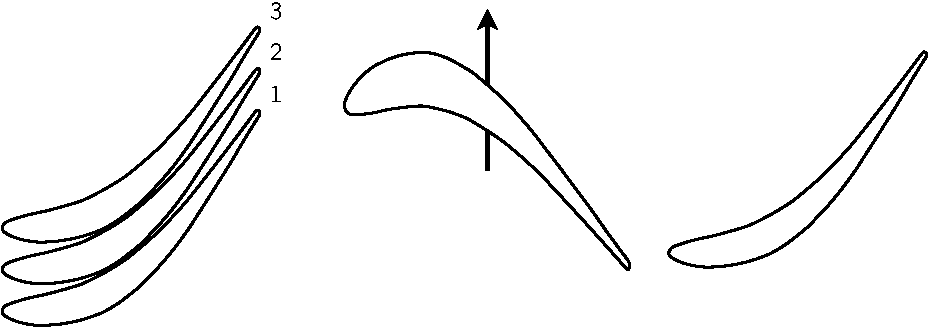
\includegraphics[width=.5\textwidth]{clocking_effect.pdf}
  \caption{Different clocking positions for a stator/rotor/stator
  configuration.}
  \label{fig:sm_nlh_clocking_effect}
\end{figure}
Fig.~\ref{fig:sm_nlh_clocking_effect} shows six
different clocking positions of the first stator
in a stator/rotor/stator configuration.
As both stator are fixed, their relative position is of 
prior interest. In fact, the wake that is generated behind the first stator
is cut by the rotor blades and transmitted to 
the stator row. The stator being fixed, the wake generated
behind the first stator is seen as a stationary wave in the second stator.
Hence, the importance of their relative position. For instance,
\citet{Huber1996} showed that
on their 1.5 turbine stage, the variation of efficiency due to clocking
effect was equal to $0.8\%$ of efficiency.

The brute force to compute the clocking effect on a
configuration is to consider all relative positions. This means
that the geometry of the stator should be rotated for each new 
clocking position. The innovative thinking proposed in 
\citet{He2002} is to consider the clocking effect as a steady wave.
In fact, as both stator are fixed, a steady perturbation
generated behind the first stator is still steady in the second stator.
In terms of frequencies, a steady perturbation is a perturbations 
whose frequency is zero. In \citet{He2002} and \citet{Vilmin2009}, 
a perturbation with zero frequency
is computed. The clocking effect can then be evaluated by
post-processing the Fourier coefficient of the zero frequency mode.
Recently, the computation of clocking effects on
arbitrary configurations has been made possible
by \citet{Vilmin2013a}.

\paragraph{Extension to the Navier-Stokes equations}
As shown above,  as the development of the non-linear harmonic
method is made in the frequency domain, applying the method to
complex equations can be difficult. For the Navier-Stokes equations,
this step is particularly hard. Nevertheless, several authors have
done this and the reader is referred to the following papers
for more information~\cite{He1998,Chen2001, He2002, Vilmin2006}.

\paragraph{Time line}
\begin{figure}[htbp]
  \centering
  \includegraphics*[scale=0.5]{timeline_nlh.pdf}
  \caption{Time line for the non-linear harmonic method}
  \label{fig:timeline_nlh}
\end{figure}
Figure~\ref{fig:timeline_nlh} shows the time line of the
development of the non-linear harmonic method. 
Note that black filled
rectangles highlight multi-frequential formulation.
\citet{He1998}
and \citet{Ning1998} first introduced the method.
\citet{He1998} developed the method for the 
two-dimensional Reynolds-Averaged Navier-Stokes equations. 
While only one harmonic is
kept in the applications, the method is presented for multiple
harmonics. It is validated on an unsteady boundary layer
on a flat plate, a transonic diffuser with oscillating back pressure
and on an oscillating transonic compressor cascade.
\citet{Ning1998} developed the method on the two-dimensional
Euler equations with moving grids 
and applied it on a transonic unsteady
channel flow and on two cascade test cases
showing a good agreement with a classical non-linear
time-marching scheme. Emphasis is put on the capability
of the non-linear harmonic method to correctly capture
the unsteadiness in presence of strong non-linearities
compared to linearized methods (presented in 
Sec.~\ref{sub:sm_lur}).
\citet{Chen2001} extended the method to the three-dimensional
Navier-Stokes equations. Stage configurations are treated and
at the interface of the stage, the perturbations are exchanged using
azimuthal Fourier transform,
the time-average field and the deterministic stresses
being flux-averaged like in a mixing-plane approach.
\citet{He2002} extended the method
to take into account for the clocking effects. The frequencies
can be chosen arbitrarily allowing its application on multi-stage
turbomachines. The clocking effect is considered as a zero-frequency
temporal wave which is actually a spatial wave. The clocking
effect is then just analyzed through a post-processing procedure.
The method is applied on a $2.5$-stage transonic
compressor. The results are analyzed in terms of clocking effects
but not compared to neither classical non-linear time marching 
computations nor analytical simulations.
\citet{Vilmin2006} implemented the method into
the commercial code Fine/Turbo. They extended the rotor-stator
interface to a non-matching join sliding mesh interface which
leads to the continuity of the unsteady flow field at the interface.
The method is validated on analytical and $2$D test cases. Finally
a $4$-stage industrial transonic compressor is simulated to prove the 
maturity of the method.
\citet{Vilmin2007} extended the method to thermally perfect gas and
applied it to a $3$D real gas flow in a radial turbine and compared their
results to a classical time-marching simulation.
\citet{Vilmin2009} implemented and validated the clocking computation method
proposed by \citet{He2002}. They validated their approach on a model problem
and applied it
on a $2$D $6.5$-stage compressor and $1.5$-stage axial turbine.
\citet{Vilmin2013a} extended the row interface to take into
account in the third rotor for perturbations 
coming from the first rotor in an
arbitrary rotor/rotor/rotor configurations.



\section{The \underline{N}on\underline{L}inear 
\underline{F}requency \underline{D}omain method (NLFD)}
\label{sub:sm_nlfd}
%!TEX root = ../../adrien_gomar_phd.tex

\paragraph{Mono-frequential formulation}

As seen before on Sec.~\ref{sub:sm_nlh}, the expansion of 
a non-linear unsteady equation in the frequency domain
can be tedious. This is even more true when the
considered equations are the Navier-Stokes equations
or any large set of non-linear equations. In
fact, the numerical schemes, the turbulence model and so
on, must be derived in the frequency domain which might be
hard to do. The NonLinear Frequency Domain approach is
proposed by \citet{McMullen2001} to overcome this issue.

To explain the development of this method, let us first 
write Eq.~\ref{eq:sm_nonlinear_convection_conservative} 
in a more general form:
\begin{equation}
	\frac{\partial u}{\partial t} + R (t) = 0,
	\label{eq:sm_nonlinear_convection_residual}
\end{equation}
with
\begin{equation}
	R(t) = \frac{\partial}{\partial x} \left( 
	\frac{u^2}{2} \right).
\end{equation}
Let us now consider that both $u$ and $R$ are periodic
in time with respect to period $T = 2 \pi / \omega$
and can be written using a Fourier series:
\begin{equation}
	\begin{split}
		u &= \sum_{k=-\infty}^{\infty} \widehat{u}_k e^{i k \omega t} \\
		R(t) &= \sum_{k=-\infty}^{\infty} \widehat{R}_k e^{i k \omega t}
	\end{split}
\end{equation}
Injecting these decompositions into 
Eq.~\ref{eq:sm_nonlinear_convection_residual} and taking into account
for the orthogonality of the complex exponentials leads to:
\begin{equation}
	i k \omega \widehat{u}_k + R_k = 0, \: k \in [-\infty, \infty]
\end{equation}
As previously, only a small number of harmonic $N$ is kept and 
a pseudo-time ($\tau$) derivative is added to march the equations
in pseudo-time to the steady-state solutions of all the harmonics:
\begin{equation}
	\fbox{$
	\displaystyle \frac{\partial \widehat{u}_k}{\partial \tau} + 
	i k \omega \widehat{u}_k + \widehat{R}_k = 0, \: k \in [-N, N]
	$}
	\label{eq:sm_nlfd_subset_eq}
\end{equation}
The fact that $R(t)$ is expressed using its own Fourier series 
makes it simpler to implement 
as it avoid developing its expression using $\widehat{u}_k^j$.
However, $\widehat{R}_k$ must be evaluated. To do so, as depicted
in Fig.~\ref{fig:nlfd_principle}, \citet{McMullen2001}
propose to use an Inverse Fast-Fourier Transform (IFFT) to get
$u(t)$ from $\widehat{u}_k^j$. Then the considered governing equation
is used to evaluate $R(t)$ which leads to $\widehat{R}_k$
through a Fast-Fourier Transform (FFT). Finally, $\widehat{u}_k^{j+1}$
is evaluated by ading the corresponding temporal derivative. All
harmonics are coupled through the IFFT and FFT operations
that needs all of them to compute the temporal signal.
\begin{figure}[htbp]
  \centering
  \includegraphics*[width=0.50\textwidth]{nlfd_principle.pdf}
  \caption{The computation of $\widehat{R}_k$ from $\widehat{u}_k$
  for the NonLinear Frequency Domain method}
  \label{fig:nlfd_principle}
\end{figure}

\paragraph{Extension to the Navier-Stokes equations}
The Navier-Stokes equations can be written in finite-volume,
semi-discrete form as:
\begin{equation}
	V \frac{\partial W}{\partial t} + R(W) = 0.
	\label{eq:navier_stokes_fv_sd}
\end{equation}
This formulation is exactly the same as the one of 
Eq.~\ref{eq:sm_nonlinear_convection_residual} meaning that
nothing particular as to be made to apply this method to
the Navier-Stokes equations. This is indeed very attractive as the
method can be applied almost directly, except for the FFT and IFFT
part that should be added into the time loop.

\paragraph{Applications}

\paragraph{Time line}
\begin{figure}[htbp]
  \centering
  \includegraphics*[width=0.40\textwidth]{timeline_nlfd.pdf}
  \caption{Time line for the NonLinear Frequency Domain method}
  \label{fig:timeline_nlfd}
\end{figure}
Figure~\ref{fig:timeline_nlfd} shows the time line of the
development of the NonLinear Frequency Domain method.
The method was first introduced by \citet{McMullen2001}
at Stanford University and applied on the two-dimensional
Navier-Stokes equations. It has been validated against an
unsteady channel flow that admits an analytical 
solution~\cite{Merkle1987} and applied to a cylinder
vortex shedding. This could be done as the frequency of the
vortex shedding was known \textit{a priori} from experimental
and numerical data. However, for a given cylinder, it is not
possible to know this frequency. This is why \citet{McMullen2002}
proposed a gradient based method for determining the period.
They applied their algorithm to find the frequency of the vortex
shedding around a cylinder.

\paragraph{Cost of the method}
The method 

% ====================
% = HARMONIC BALANCE =
% ====================
\section{The \underline{H}armonic \underline{B}alance method (HB)}
\label{sec:sm_hb}
%!TEX root = ../../adrien_gomar_phd.tex

The HB method has been originally
proposed by \citet{Hall2002}, at that time named
Harmonic Balance Technique (HBT).
It is a step further the non-linear frequency domain method. Instead
of using the fast Fourier transform to cast back the equations
to the time domain at each pseudo-iteration step, 
the equations are mathematically derived to be directly
computed into the time-domain.
To explain the method, we will again use the general form of 
the non-viscous Burger's equation as defined in
Eq.~\eqref{eq:sm_nonlinear_convection_residual}.


\subsection{Mono-frequential formulation}

Following the same approach as the non-linear frequency domain one,
consider that both $u$ and $R$ are periodic
in time with respect to period $T = 2 \pi / \omega$
and can be written using a Fourier series:
\begin{equation}
	\begin{split}
		u(t) &= \sum_{k=-\infty}^{\infty} \widehat{u}_k e^{i k \omega t}, \\
		R(t) &= \sum_{k=-\infty}^{\infty} \widehat{R}_k e^{i k \omega t}.
		\label{eq:sm_hall_dft}
	\end{split}
\end{equation}
Injecting Eq.~\eqref{eq:sm_hall_dft} in 
Eq.~\eqref{eq:sm_nonlinear_convection_residual}, and considering
the orthogonality of the complex exponentials:
\begin{equation}
	i k \omega \widehat{u}_k + \widehat{R}_k = 0, \: k \in [-N, N].
	\label{eq:sm_hall_frequential_eq}
\end{equation}

In the same way as one uses Fourier coefficients to
evaluate the temporal signal,
one can reconstruct the Fourier coefficients using
temporal evaluations. These are taken at evenly spaced timelevels
sampling the period $T = 2 \pi / \omega$ using the forward
Fourier transform. Moreover, 
according to the Nyquist-Shannon~\cite{Shannon1949} sampling theorem, 
at least $2N$ timelevels are needed to capture $N$ frequencies. Actually
$2N+1$ timelevels are used to prevent from odd-even decoupling as
demonstrated by \citet{Weide2005}. $\widehat{u}_k$ can thus
be expressed in function of $u(t)$:
\begin{equation}
	\widehat{u}_k = \frac{1}{2N+1} 
	\sum_{n=0}^{2N} u(t_n) e^{-i k \omega t_n}.
\end{equation}
If $E$ denotes the matrix composed of the elements 
$(E)_{k,n} = e^{-i (k - N) \omega t_n} / 2N+1$, one can write $\widehat{u}_k$
and $\widehat{R}_k$ as:
\begin{equation}
	\begin{split}
		\widehat{u}_k &= E u^\star, \\
		\widehat{R}_k &= E R^\star.
	\end{split}
	\label{eq:sm_matrix_fourier_operator}
\end{equation}
where $u^\star$ and $R^\star$ 
denote the vectors formed of all the evaluations of respectively $u$
and $R$,
made at $2N+1$ timelevels uniformly sampling the period of interest:
\begin{equation}
	\begin{split}
		u^\star &= [u(t_0), \ldots, u(t_{2N})], \\
		R^\star &= [R(t_0), \ldots, R(t_{2N})].
	\end{split}
\end{equation}
$E$ can thus be named the Fourier matrix.
Note that conversely, using the inverse Fourier matrix $E^{-1}$:
\begin{equation}
	\begin{split}
		u^\star &= E^{-1} \widehat{u}_k \\
		R^\star &= E^{-1} \widehat{R}_k.
	\end{split}
\end{equation}
Injecting the matrix formulation of 
Eq.~\eqref{eq:sm_matrix_fourier_operator} in 
Eq.~\eqref{eq:sm_hall_frequential_eq}
gives:
\begin{equation}
	i \omega K E u^\star + E R^\star = 0,
\end{equation}
where $K$ is a diagonal matrix formed of all the $k \in [-N, N]$.
Note that first, the matrix formulation encompass all harmonics
$k \in [-N, N]$ and second, it does not require the
orthogonality of the complex exponentials.
Now multiplying the equation by the inverse Fourier matrix $E^{-1}$:
\begin{equation}
	i \omega E^{-1} K E u^\star + R^\star = 0,
	\label{eq:sm_hb_matrix_form_mono}
\end{equation}
where $R^\star$ can now be substituted:
\begin{equation}
		i \omega E^{-1} K E u^\star + 
		\displaystyle \frac{\partial}{\partial x}
		\frac{(u^\star)^2}{2} = 0.
\end{equation}
What happened here is that instead of developing $R(t)$
in the frequency domain as made in the NLH approach,
which is tedious, this term is kept
in this form through all the development process. 
Since $R(t)$ only includes spatial derivatives, no non-linear
terms
arise by using the Fourier decomposition. Thus, multiplying it
by the Fourier matrix leads to the unity matrix. 
$R(t)$ is then simply evaluated at $2N+1$ timelevels.

This approach is really close to the NLFD method.
The higher order perturbation terms are taken into account
in the equations.
The reader might observe that we are introducing the discrete Fourier
transform and its inverse. This is close to the fast Fourier transform
and its inverse, as proposed by \citet{McMullen2001}. However,
as the development is on the equations and not during the time loop,
we get $2N+1$ steady equations, by definition in the time
domain, that are coupled by a source term.
The main difference with the NLFD approach
is that the source term is known at the first iteration and does
not change, meaning that we do not spend time computing a
fast Fourier transform and its inverse at each time-step.
The source term appears as a spectral operator defined as:
\begin{equation}
	D_t = i \omega E^{-1} K E.
	\label{eq:sm_hb_mono_source_term_matrix}
\end{equation}

\citet{Gopinath2005} named the HB approach the 
Time Spectral Method (TSM) and provided 
an analytical formulation of the
source term defined in Eq.~\eqref{eq:sm_hb_mono_source_term_matrix}.
It is a matrix operator whose elements are defined as:
\begin{equation}
  (D_t)_{k, n} =
  \begin{cases}
    \frac{\pi}{T}(-1)^{k-n}\csc\left(\frac{\pi
        (k-n)}{2N+1}\right) &, \, k\neq n,\\
    0 &, \, k=n.
  \end{cases}
  \label{eq:sm_hb_mono_source_term_analytic}
\end{equation}
Finally, adding a pseudo-time ($\tau$) derivative to 
time march the equations to the steady state, 
the mono-frequential formulation of 
Eq.~\eqref{eq:sm_nonlinear_convection_conservative} in the harmonic
balance framework is given by:
\begin{equation}
	\fbox{$
	\displaystyle \frac{\partial u^\star}{\partial \tau} + 
	D_t (u^\star) + 
	\displaystyle \frac{\partial}{\partial x}
		\frac{(u^\star)^2}{2} = 0.
	$}
\end{equation}
with $D_t$ defined using Eq.~\eqref{eq:sm_hb_mono_source_term_analytic}.

\subsection{Multi-frequential formulation}
\citet{Gopinath2007} and \citet{Ekici2007} 
extended the harmonic balance approach to
a multi-frequential formulation. To do so, they considered
a Fourier matrix defined as:
\begin{equation}
	(E)_{k,n} = \frac{1}{2N+1} e^{-i \omega_{k-N} t_n},
\end{equation}
where $N$ is the chosen number of frequencies.
Note that replacing $\omega_{k-N}$ by $(k - N) \omega$ gives
the mono-frequential inverse Fourier matrix back. 
This can be justified mathematically: in the
framework of the almost-periodic functions~\cite{Besicovitch1932},
such a function (which is composed of multiple
frequencies non necessarily harmonically related) can be approximated
by an almost-periodic
discrete Fourier transform. If $f(t)$ is an almost-periodic function,
\citet{Besicovitch1932} proves that it can be approximated as:
\begin{equation}
	f(t) \approx \sum_{k=-N}^{N} \widehat{f}_k 
	e^{i \omega_k t}.
\end{equation}
This allows the use of the multi-frequential Fourier matrix as defined
above. However, in the multi-frequential case, the inverse Fourier matrix
$E^{-1}$ is not known \textit{a priori} 
and has to be numerically computed. Actually, as demonstrated by 
\citet{Gopinath2007}, it is easier to expressed $E^{-1}$ analytically,
compute its temporal derivative (that is hence analytical too) 
and inverse it numerically to obtain $E$.

Using the same process as for the mono-frequential formulation,
Eq.~\eqref{eq:sm_nonlinear_convection_residual} becomes:
\begin{equation}
	i E^{-1} P E u^\star + R^\star = 0,
\end{equation}
where $P$ is a diagonal matrix formed of all the pulsations $\omega_k$.
Note that the exponentials do not need to be form an
orthogonal family here. The only need is to have the multi-frequential
Fourier matrix $E$ to be invertible.
This is really close to the mono-frequential formulation given
in Eq.~\eqref{eq:sm_hb_matrix_form_mono}.
Finally, adding a pseudo-time ($\tau$) derivative 
to time-march the equation to the steady state,
the multi-frequential formulation of 
Eq.~\eqref{eq:sm_nonlinear_convection_conservative} in the harmonic
balance framework reads:
\begin{equation}
	\fbox{$
	\displaystyle \frac{\partial u^\star}{\partial \tau} +
	D_t (u^\star) + 
	\displaystyle \frac{\partial}{\partial x}
		\frac{(u^\star)^2}{2} = 0.
	$}
\end{equation}
with $D_t$ defined as:
\begin{equation}
	D_t = i E^{-1} P E,
\end{equation}
and again $u^\star = [u(t_0), \ldots, u(t_{2N})]$ 
and $R^\star = [R(t_0), \ldots, R(t_{2N})]$.

For the mono-frequential formulation, the use of a uniform
sampling of the timelevels has the good property of being
well conditioned.
Before go into details, let us recall the definition of the
condition number $\kappa$ of a matrix $E$:
\begin{equation}
	\kappa (E) = \kappa (E^{-1}) = \| E \| \cdot \| E^{-1} \|, \quad
    \kappa(E) \geq 1,
\end{equation}
where $\| \cdot \|$ denotes a matrix norm.  Considering the resolution
of the system of equation
$A x = b$, if $A$ is invertible and if $\delta A$, $\delta x$ and
$\delta b$ are the numerical errors associated with the computation of
$A$, $x$ and $b$, respectively, then:
\begin{equation}
   (A + \delta A)(x + \delta x) = b + \delta b.
   \label{eq:error_reso}
\end{equation}
By definition, the condition number sets an upper bound for 
the error made on~$x$:
\begin{equation}
   \frac{\| \delta x \|}{\| x \|} \leq 
   \kappa(A)\left[\frac{\| \delta A \|}{\| A \|} + 
   \frac{\| \delta b \|}{\| b \|} \right].
   \label{eq:conditonnig_amp}
\end{equation}
The error on the iterative resolution of the governing equations can
therefore be amplified by the harmonic balance source term. 
This amplification is
led by the condition number of the multi-frequential Fourier matrix. This
also means that if the error is small but the condition number is
high, and vice-versa, the computation can diverge too. However, the
error can not be \emph{a priori} controlled, thus the need to
minimize the condition number.

In the mono-frequential formulation, 
the Fourier matrix is well-conditioned: the
uniform sampling for harmonically related frequencies leads to a
condition number equal to~$1$, which is the theoretical lower bound
for the condition number.  This is linked to the orthogonality of the
complex exponential family.  On the other hand, when the frequencies are arbitrary, it is usually
impossible to choose a uniform set of time instants over which the
multi-frequential Fourier matrix~$E$ is well conditioned. In fact, it is common for uniformly-sampled
sinusoids at two or more frequencies to be nearly linearly dependent,
which causes them not to be orthogonal, leading to the
ill-conditioning encountered in practice. This issue will be discussed
further in Sec.\mytodo{sec conditinnning} and an innovative
solution will be proposed.

\subsection{Extensions}

\paragraph{Navier-Stokes equations}
Equivalent to the NLFD method, the
considered equation is really close to the finite-volume
semi-discrete form of the Navier-Stokes equations. Therefore,
nothing particular has to be made to apply the harmonic balance approach
to the Navier-Stokes equations.
This shows its advantage over the NLFD and particularly over the NLH method.

\paragraph{Turbomachinery computations}
Originally, the HB method has been developed for 
turbomachinery applications.
\citet{Hall2002} applied the method to the computation
of flutter boundary in front stage transonic rotor 
of a modern high-pressure compressor. To reduce the
computational domain to a single blade passage, 
a phase-lagged boundary condition is used at the azimuthal
interfaces:
\begin{equation}
	\widehat{u}_{k, U} = \widehat{u}_{k, L} e^{i \beta k},
\end{equation}
for $k \in [-N, N]$, where subscript $U$ and $L$ denotes
respectively the upper and lower parts of the azimuthal boundaries.
$\beta$ denotes the inter-blade phase angle. This boundary
condition allows to compute isolated aero-elastic configurations
using only one blade-passage.
\citet{Weide2005} extended the approach to take into account
for periodic boundary conditions when the equations are solved in the
cartesian coordinate system. The efficiency of the
method is demonstrated on the NASA-Stage~$35$ and shows that
engineering accuracy is obtained with only $N=5$ harmonics.
Nothing is said on the strategy used at the rows interface.
\citet{Ekici2007} and \citet{Gopinath2007}
extended the method to a muti-frequential formulation. 
As such, it can then be applied to multi-stage
configurations. Both of them demonstrated the application of
the method to
a two-dimensional multi-stage compressor called
configuration D. 
The strategy used by \citet{Ekici2007} 
to exchange the variables at
the rows interface is schematically represented 
in Fig.~\ref{fig:bnd_sliding_ekici2007}.
The temporal and azimuthal variation 
of the field (here represented as $u (\theta_i, t_i)$)
in row $i$ is first temporally Fourier transformed, and then
spatially to obtain the spatio-temporal modes $\widetilde{u}_i$.
At the interface, these modes are transmitted using a non-reflecting
boundary condition filtering the spurious modes. In fact, as only some
temporal modes are computed using the HB approach, only
those will be kept when transmitted at the opposite row.
Finally, the inverse operations are carried out: first an inverse
azimuthal Fourier transform is performed and second an inverse
temporal Fourier transform is done which gives $u (\theta_j, t_j)$
in row $j$.
\begin{figure}[htbp]
  \centering
  \includegraphics*[scale=0.25]{bnd_sliding_ekici2007.pdf}
  \caption{Exchange of the variable at rows interface as described by \citet{Ekici2007}.}
  \label{fig:bnd_sliding_ekici2007}
\end{figure}
\citet{Gopinath2007} used a different approach to transfer
the information at the interface as depicted
in Fig.~\ref{fig:bnd_sliding_gopinath2007}. In most time-domain solver,
a sliding mesh treatment exists to interpolate azimuthal variations
between consecutive rows. Therefore, \citet{Gopinath2007}
interpolates temporally the field on the time samples
of the opposite row. To do so, they used a temporal Fourier
transform combined with an inversed one.
Then, they applied the sliding mesh treatment
to spatially transfer the information. Again, as spurious effects
can appear, the time interpolation is done, not on the $2N+1$ samples
of the opposite row, but rather on $2\cdot (2N+1)$ samples. This over-sampling
helps isolating the spurious effects on the higher harmonics to suppress them.
\begin{figure}[htbp]
  \centering
  \includegraphics*[scale=0.25]{bnd_sliding_gopinath2007.pdf}
  \caption{Exchange of the variable at rows interface as described by \citet{Gopinath2007}.}
  \label{fig:bnd_sliding_gopinath2007}
\end{figure}
\citet{Ekici2008a} applied the multi-frequential method
to the effect of wake passing on the vibration of
a turbine blade. Note that the stator is modeled
by an unsteady wake injection but not computed.
Two frequencies are involved: the blade passing
frequency of the opposite row, here the
stator row that is modeled through an unsteady wake injection,
and the aero-elastic frequency, justifying the use
of the multi-frequential formulation.
\citet{JSicot2012} adapted the harmonic balance 
to phase-lag periodic 
conditions to reduce the computational domain
and gave the general expression of the phase-lag due to
different number of blades in the different rows:
\begin{equation}
 	\beta = - 2 \pi \sign \left(\Omega_{cur} - \Omega_{opp} \right) 
 	\left(1 - \frac{B_{opp}}{B_{cur}}\right),
\end{equation} 
where $\Omega$ denotes the rotation speed, $B$ the number
of blade, subscript $opp$ and $cur$ denotes respectively the
opposite and the current row.
A row coupling strategy is set up, it involves 
a time and space interpolation at row interfaces.
A filter is applied to remove spurious waves.
\citet{JGuedeney2013} applied the multi-frequential
formulation to the computation of a $1.5$ stage subsonic
compressor.
Then, \citet{JSicot2013} applied it to a $3$D
$3.5$ stage industrial compressor, proving the maturity of
the method.

\paragraph{Aeroelastic simulations}
\citet{Thomas2002a} used the method to
determine the limit-cycle oscillation solution
of a transonic airfoil configuration using the
Euler equations and \citet{Thomas2004b} extended
it to the viscous Navier-Stokes equations.
\citet{JDufour2009} highlight the benefits of using a 
non-linear approach for oscillating-flap simulations
compared to linearized approaches. A one-harmonic HB simulation
gives results comparable to an expensive time-marching simulation.
\citet{Huang2013} applied the mono-frequential
HB method to the flutter prediction of the 
$11\textsuperscript{th}$ 
standard configuration for aeroelasticity~\cite{Fransson1999}.
They show that with only one harmonic, the local
harmonic response of the fluid is superimposed
to the results of a time-marching simulation.
The same study has been performed by 
\citet{Jsicot12:_time_domain_harmon_balan_method}
and shows the same conclusions.
\citet{JSicot2013} applied the multi-frequential 
method to the
aeroelasticity of a contra-rotating fan, proving
the maturity of the method. The same type of 
computations will be run in this thesis.


\paragraph{Transient problems}
\citet{Mavriplis2012} extended the method to 
an hybrid polynomial/harmonic balance approaches. 
It allows to use the method for maneuver simulations, 
where a part of the simulation exhibits a physical transient.
The method is also extended to overlapping mesh grids.

\paragraph{Time sampling in the case of multi-frequential formulation}
\citet{Gopinath2007} and \citet{Ekici2007}
applied the multi-frequential method to
a two-dimensional multistage compressor called
configuration D. \citet{Ekici2007} use
$3N+1$ evenly spaced 
timelevels to improve the condition number
of the source term while \citet{Gopinath2007}
stays with $2N+1$ evenly spaced timelevels.
\citet{Ekici2008a} applied the multi-frequential method
to the effect of wake passing on the vibration of
a turbine blade and uses $2N+1$ evenly spaced
timelevels are considered.
\citet{JGuedeney2013} introduce non-uniform 
timelevels to minimize the condition number of multi-frequential
computations. 
The effect of the condition number on the stability
of the computations is assessed along with algorithms
to optimize the choice of the timelevels.
This allows to drastically reduce the condition number for
any combination of frequencies, 
while keeping only $2N+1$ samples.
The method is then applied
to a $1.5$ stage subsonic compressor.
Note that a part of this work has been done in this
thesis and will be detailed latter on.

\paragraph{Gradient-based method to determine the frequency}
With the same approach as \citet{McMullen2002}, \citet{Gopinath2006}
developed a gradient-based method to estimate the frequency of a 
vortex shedding behind a cylinder and a NACA0012 airfoil 
at high angle of attack using the harmonic balance approach.

\paragraph{Optimum shape design}
\citet{Thomas2005b} used an automatic 
differentiation software tool to derive an adjoint code
from a harmonic balance code and validated this approach
on a representative model problem.

\paragraph{Adaptive method}
\citet{Maple2004} presented an adaptive harmonic
balance approach. The number of harmonics is increased
if the energy of the last harmonic divided by the cumulative
sum of the energy of each harmonic is larger than a 
given threshold. During the first iterations, only
a low number of harmonic is kept. Then, when the flow
is almost converged, the adaptive harmonic balance
approach is used. This ensures that higher order harmonics
are not injected at the first iterations, when the
flow is not physical. A $86\%$ reduction in time (and
in memory footprint) is seen compared to a resolved (converged in
terms of harmonics $N$) harmonic
balance computation. This has to be compared to
the $2$ factor speed-up observed by \citet{Mosahebi2013}
with an adaptive NLFD approach.

\subsection{Cost of the method}
As mentioned before, the cost of the method is linked to
the number of timelevels simulated.
In fact, each new timelevel corresponds to an additional steady computation.
Thus, if $2N+1$ timelevels are considered and if $\mathdollar_{\text{RANS}}$ 
denotes the CPU and memory cost of
one steady computation, the cost of the HB method can be 
approximated by:
\begin{equation}
	\mathdollar_{\text{HB}} = (2N+1) \cdot \mathdollar_{\text{RANS}}.
\end{equation}
Note that \citet{Ekici2007,Ekici2008a} use $3N+1$
timelevels or more due to solve the bad conditioning of the
source term. Thus, in that
case, the cost is bigger and scales with the chosen number
of timelevels.

% ===================================
% = Periodic flows in turbomachines =
% ===================================
\section{Periodic flows in turbomachines}
\label{sec:sm_hudson}
%!TEX root = ../../adrien_gomar_phd.tex

As said in the introduction, the relative
velocity between two consecutive rows induces
unsteadinesses that can be correlated with the 
Blade Passing Frequency (BPF). A 

\chconclu{Four spectral methods have been presented in this chapter.
The main mathematical development have been demonstrated and 
the hypothesis/weakness of each method has been highlighted.
In particular, the presented harmonic balance method can
treat both mono and multi-frequential applications. One
unsteady equation is transformed into a subset of $2N+1$
steady-state equations coupled by a source term. This last
is analytical in the mono-frequential formulation and
of matrix form in the multi-frequential framework.
The large literature available on these methods shows that
they are ready for industrial, numerically hard
unsteady applications. Moreover, the method is able to
efficiently compute aeroelastic phenomenon on 
contra-rotating configurations explaining its
use in the present thesis.}
